\documentclass{beamer}

\usepackage[latin1]{inputenc} % can be changed to utf8x
\usepackage[T1]{fontenc}
\usepackage[french]{babel}
\usepackage{lmodern}
\usepackage{color}
\usepackage{listings}
\usepackage{svg}
\usepackage{appendixnumberbeamer}
\usepackage{hyperref}


\usepackage{booktabs}
\usepackage[scale=2]{ccicons}

\usepackage{pgfplots}
\usepgfplotslibrary{dateplot}

\usepackage{xspace}
\newcommand{\themename}{\textbf{\textsc{metropolis}}\xspace}
\definecolor{orange}{rgb}{1,0.5,0}

\lstdefinelanguage{python}
{morekeywords=[1]{import,from,False,True,and,or,not,if,else,elif,while,break,continue,def,return,global,in,None,for,class,is,try,except,pass,assert,lambda,raise,yield,nonlocal,with,as,cdef,extern},
morekeywords=[2]{complex,str,int,set,dict,frozenset,list,float},
morekeywords=[3]{print,type,sqrt,input,sin,len,del,range,namedtuple,radians,chr,isinstance,zip,map,filter,sum,all,any,iter,next,callable,open},
morekeywords=[4]{@property},
morekeywords=[5]{OSError,StopIteration,IndexError,ValueError,IOError},
morestring=[b]{"},
morestring=[b]{'},
morestring=[b]{"""},
morecomment=[l]{\#},}[keywords,comments,strings,directives]

% Listing style
\lstset{basicstyle=\fontsize{7}{8}\selectfont\tt}
\lstset{keywordstyle=[1]\color[rgb]{0,0,1}\bfseries}
\lstset{keywordstyle=[2]\color[rgb]{0.6,0,0}\bfseries}
\lstset{keywordstyle=[3]\color[rgb]{0,0.6,0}\bfseries}
\lstset{keywordstyle=[4]\color{orange}\bfseries}
\lstset{keywordstyle=[5]\color[rgb]{0.463,0.294,0.557}\bfseries}
\lstset{directivestyle=\color[rgb]{0.314,0.40,0.565}\bfseries}
\lstset{identifierstyle=\color{black}}
\lstset{commentstyle=\color[rgb]{0,0.6,0.6}}
\lstset{stringstyle=\color[rgb]{0.44,0.47,1}}
\lstset{stringstyle=\color[rgb]{0.44,0.47,1}}
\lstset{showstringspaces=false,showtabs=false,tabsize=3,extendedchars=true,breaklines=true,postbreak={},breakautoindent=true,breakindent=0pt}
\lstset{frame=shadowbox,rulecolor=\color[gray]{.2},rulesepcolor=\color[gray]{.75},framesep=2pt,backgroundcolor=\color[rgb]{1,1,0.9}}
\lstset{xleftmargin=0.1cm,xrightmargin=1mm,aboveskip=0.5cm,belowskip=0cm}
\lstset{captionpos=b,numbers=left,numberstyle=\tiny,columns=fixed,escapechar=§}
\lstset{language=python}

\usetheme{metropolis}           % Use metropolis theme
\title{Decorator Design Pattern}
\date{\today}
\author{Jonathan Petit}
\institute{ECAM}
\begin{document}
  \maketitle

\section{The Decorator design pattern}

  \begin{frame}{Context and application}
    \frametitle{Context and application}
    \begin{itemize}
      \item Attach \textcolor{red}{features dynamically} \\
      \textit{Add new functionality to an existing object without altering its structure.}
      \item \textcolor{red}{Single responsibility} principle. \\
      \textit{Divide functionality between classes with unique feature.}
      \item \textcolor{red}{Embellishment} of a core object by recursively wrapping \\
      \textit{Basic object is envelloped with its different characteristics.}
    \end{itemize}
  \end{frame}

  \begin{frame}{Bad Structure}
    \frametitle{Bad structure}
    \begin{itemize}
      \item A base class \textcolor{red}{"Windows"} \\
      \textit{A new class inherited when a new windows have others options.}
      \item A lot of \textcolor{red}{repetition} \\
      \textit{The classes have a lot of resemblance.}
    \end{itemize}
    \begin{figure}[!b]
      \centering
      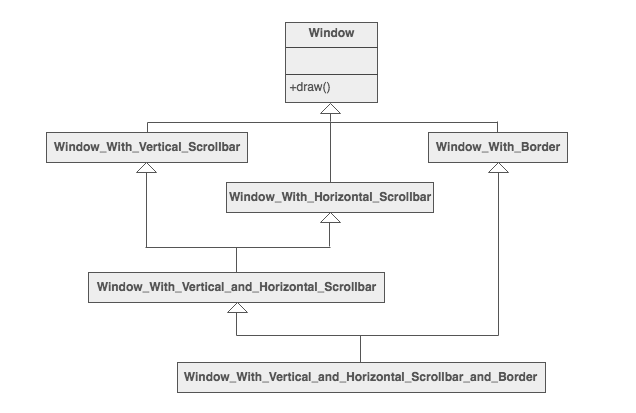
\includegraphics[scale=0.25]{bad}
      \caption{Bad structure}
    \end{figure}
  \end{frame}

  \begin{frame}{Good structure}
    \frametitle{The solution structure}
    \begin{itemize}
      \item A base class (interface)
      \item Few concretes classes of the base class
      \item A decorator class
      \item Few options
    \end{itemize}
    \begin{figure}[!b]
      \centering
      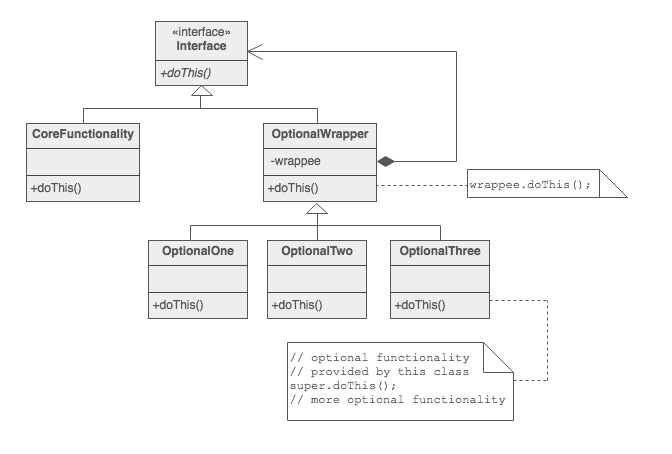
\includegraphics[scale=0.27]{good}
      \caption{The Decorator design pattern}
    \end{figure}
  \end{frame}

  \begin{frame}{Base class}
    \frametitle{The base class(1)}
    \begin{itemize}
      \item The \textcolor{red}{basic representation} of an object \\
      \textit{Without the characteristics of the options.}
    \end{itemize}
    \begin{figure}[!b]
      \centering
      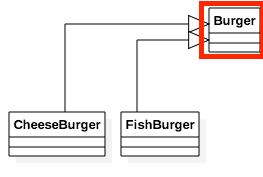
\includegraphics[scale=0.4]{Base}
      \caption{The base class}
    \end{figure}
  \end{frame}

  \begin{frame}{Base class}
    \frametitle{The base class(2)}
    \lstinputlisting[firstline=0,lastline=11]{../scr/decorator.py}
  \end{frame}

  \begin{frame}{Concrete class}
    \frametitle{The concrete class(1)}
    \begin{itemize}
      \item The representation of a \textcolor{red}{concrete object} \\
      \textit{Inheritance of the basic object.}
      \item \textcolor{red}{Specification} of the main class \textbf{Burger} \\
      \textit{Object with its own characteristics.}
    \end{itemize}
    \begin{figure}[!b]
      \centering
      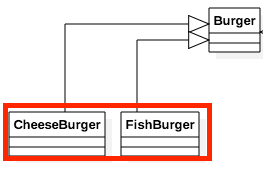
\includegraphics[scale=0.4]{concrete}
      \caption{The concretes classes}
    \end{figure}
  \end{frame}

  \begin{frame}{Concrete class}
    \frametitle{The concrete class(2)}
    \lstinputlisting[firstline=14,lastline=30]{../scr/decorator.py}
  \end{frame}

  \begin{frame}{Decorator class}
    \frametitle{The decorator class(1)}
    \begin{itemize}
      \item An \textcolor{red}{abstract class} of the basic object \textbf{Burger} \\
      \textit{Encapsulation of the original object inside an abstract wrapper interface.}
      \item Giving \textcolor{red}{the abilities} to specify \\
      \textit{Abstract class to attach a combination of features at concrete class.}

    \end{itemize}
    \begin{figure}[!b]
      \centering
      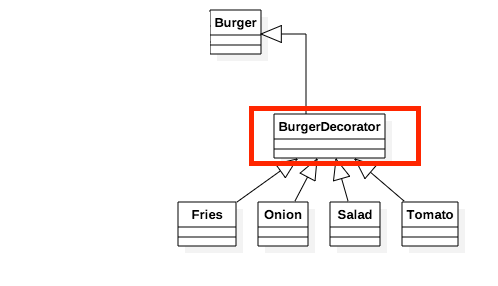
\includegraphics[scale=0.27]{Decorator}
      \caption{The decorator class}
    \end{figure}
  \end{frame}

  \begin{frame}{Decorator class}
    \frametitle{The decorator class(2)}
    \lstinputlisting[firstline=33,lastline=47]{../scr/decorator.py}
  \end{frame}

  \begin{frame}{Options classes}
    \frametitle{The options classes(1)}
    \begin{itemize}
      \item The features to \textcolor{red}{wrap} a concrete object\\
      \textit{Inheritance of the abstract class decorator.}
    \end{itemize}
    \begin{figure}[!b]
      \centering
      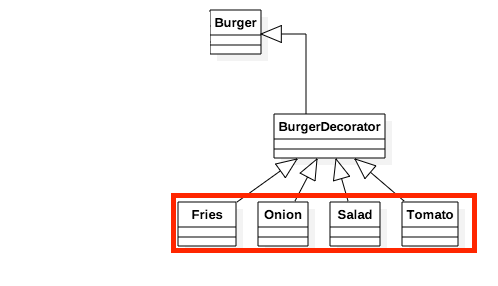
\includegraphics[scale=0.4]{options}
      \caption{The options classes}
    \end{figure}
  \end{frame}

  \begin{frame}{Options classes}
    \frametitle{The options classes(2)}
    \lstinputlisting[firstline=49,lastline=68]{../scr/decorator.py}
  \end{frame}

  \begin{frame}{Example}
    \frametitle{Example(1)}
    \lstinputlisting[firstline=77,lastline=83]{../scr/decorator.py}
    \begin{itemize}
      \item CheeseBurger sauce Ketchup
      \item CheeseBurger sauce Ketchup with tomato
      \item FishBurger sauce Tartar with salad tomato fries
    \end{itemize}
  \end{frame}

  \begin{frame}{Options classes}
    \frametitle{Example(2)}
    \begin{itemize}
      \item The \textcolor{red}{complete diagram} of the application\\
      \textit{The main class \textbf{Burger} with concrete classes and the options to wrap and decorate concrete classes.}
    \end{itemize}
    \begin{figure}[!b]
      \centering
      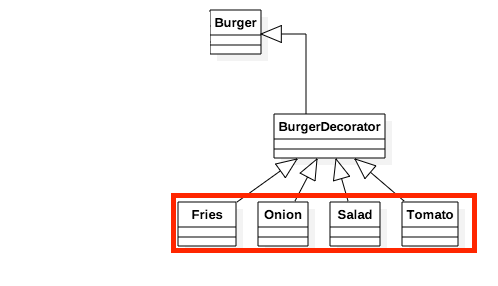
\includegraphics[scale=0.4]{Burger}
      \caption{The complete diagram}
    \end{figure}
  \end{frame}

  \begin{frame}{Application}
    \frametitle{Application}
    \begin{itemize}
      \item Output of the little application (main.py)\\
    \end{itemize}
      \begin{figure}
        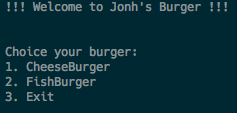
\includegraphics[width=3cm, height=2cm]{first}
        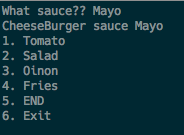
\includegraphics[width=3cm, height=2cm]{second}
        \caption{The menus of main.py (cf: GitHub)}
      \end{figure}
      \begin{figure}[!b]
        \centering
        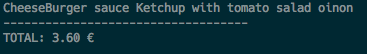
\includegraphics[scale=0.4]{third}
        \caption{The ouput of main.py (cf: GitHub)}
      \end{figure}

  \end{frame}

  \begin{frame}{Conclusion}
    \frametitle{Conclusion}
    The decorator pattern used when:
    \begin{itemize}
      \item A base object have \textcolor{red}{multiple derivates} \\
      \textit{A \textbf{Burger} may be a \textbf{CheeseBurger} or \textbf{FishBurger}.}
      \item Derivates may be wrap with \textcolor{red}{same or differentes features} \\
      \textit{\textbf{CheeseBurger} with tomato or \textbf{FishBurger} with salad and tomato.}
      \item Decorator pattern \textcolor{red}{allows to add} new derivates or options easily \\
      \textit{A new concrete class \textbf{VegetarianBurger} or a new option \textbf{pickels}.}
    \end{itemize}
  \end{frame}

  \appendix

  \begin{frame}{Enjoy!}
    The application burger is available on GitHub:
    \begin{itemize}
      \item \url{https://github.com/JonathanPetit/Decorator-design-pattern}
      \item The manual is the README.md
    \end{itemize}
  \end{frame}

  \begin{frame}[allowframebreaks]{Bibliography}
    \begin{thebibliography}{9}
      \setbeamertemplate{bibliography item}[online]
      \bibitem{A} \url{https://sourcemaking.com/design_patterns/decorator}
      \setbeamertemplate{bibliography item}[online]
      \bibitem{A} \url{https://en.wikipedia.org/wiki/Decorator_pattern}
      \setbeamertemplate{bibliography item}[online]
      \bibitem{A} \url{https://www.tutorialspoint.com/design_pattern/decorator_pattern.htm}
      \setbeamertemplate{bibliography item}[book]
      \bibitem{B} Architecture logiciel slides - Mr. Comb\'efis
      \setbeamertemplate{bibliography item}[online]
      \bibitem{B} \url{https://github.com/matze/mtheme}

    \end{thebibliography}
  \end{frame}

\end{document}
